\chapter{Blokové plány}

\section{Definícia, základné vlastnosti}

\begin{definition}

Vyvážený nekompletný blokový plán (angl. \emph{balanced incomplete block design}) $BIBD(v, b, r, k, \lambda)$ je usporiadaná dvojica $(X, \mathcal{B})$, kde $X$ je množina objektov a $\mathcal{B} \subset \powerset(X)$ je množina podmnožín objektov (tieto podmnožiny voláme \emph{bloky}), pričom sú splnené nasledujúce podmienky:

\begin{enumerate}
    \item $v = |X|$ je mohutnosť množiny objektov.
    \item $b = |\mathcal{B}|$ je mohutnosť množiny blokov.
    \item každý blok má mohutnosť $k$.
    \item každý bod je obsiahnutý v práve $r$ blokoch.
    \item každá dvojica bodov sa vyskytuje v práve $\lambda$ blokoch. 
\end{enumerate}
\end{definition}

\begin{theorem}
$\exists BIBD(v, b, r, k, \lambda) \Longleftrightarrow $ $\lambda$-násobný kompletný multigraf rádu~$v$ $\lambda K_v$
sa dá rozložiť na $b$ hranovo disjunktných klík rádu~$k$ ($K_k$).
\end{theorem}


\begin{proof}
Množina objektov $X$ zodpovedá množine vrcholov multigrafu. 
Výskyt dvojice objektov v bloku zodpovedá hrane v multigrafe.
Samotné bloky zodpovedajú kompletným klikám.

Formálna konštrukcia je z toho očividná.
\end{proof}

\begin{theorem}
\label{th:bibd_params}
Nech existuje $BIBD(v, b, r, k, \lambda)$. Potom:
\begin{enumerate}
    \item $vr = bk$
    \item $\lambda (v-1) = r (k-1)$
\end{enumerate}
\end{theorem}


\begin{exercise}
Dokážte vetu \ref{th:bibd_params}. \emph{Hint: prvá rovnosť vyjadruje celkový počet bodov vo všetkých blokoch (s opakovaním), druhá rovnosť vyjadruje celkový počet hrán pre jeden vrchol v zodpovedajúcom multigrafe.}
\end{exercise}

\begin{corollary}
Preto namiesto značenia $BIBD(v, b, r, k, \lambda)$ budeme často
použivať značenie $BIBD(v, k, \lambda)$, nakoľko 
zvyšné parametre vieme dorátať: 
$$r := \dfrac{\lambda (v-1)}{k-1},~ b := \dfrac{\lambda v (v-1)}{k (k-1)}$$
\end{corollary}

\begin{theorem}

Nech existuje $BIBD(v, b,r, k, \lambda)$, kde $X = \set{x_1, x_2, \ldots, x_v}$ a $\mathcal{B} = \set{B_1, \ldots, B_b}$. 
Nech matica incidencie $A \in \set{0, 1}^{v \times b}$ je matica typu $v\times b$, kde $A_{ij} = 1$ práve vtedy, keď $x_i \in B_j$.
Potom $A A^T = (r-\lambda) I_v + \lambda J_{v}$, kde $I_v$ je matica identity rádu $v$ a $J_v$ je matica jednotiek typu $v \times v$.
\end{theorem}

\begin{proof}
Pozrieme sa na jednotlivé políčka matice $A A^T$:
\begin{equation*}
(AA^T)_{ik} = \sum_{j=1}^b (A)_{ij} (A^T)_{jk} = \sum_{j=1}^b (A)_{ij} (A)_{kj} = \sum_{j=1}^b [x_i \in B_j] [x_k \in B_j] = \sum_{j=1}^b [x_i \in B_j \wedge x_k \in B_j]
\end{equation*}
Slovne povedané, políčko $(AA^T)_{ik}$ sa rovná počtu blokov, kde sa naraz vyskytujú prvky $x_i$ a $x_k$.
V prípade, že $i = k$, $(AA^T)_{ik} = r$, nakoľko sa v blokovom pláne každý prvok vyskytuje v práve $r$ blokoch.
V opačnom prípade $(AA^T)_{ik} = \lambda$, nakoľko sa každá dvojica prvkov v blokovom pláne vyskytuje v práve $\lambda$ blokoch.

Čiže matica $AA^T$ má na diagonále číslo $r$ a mimo diagonály číslo $\lambda$, čo presne vyjadruje vzorec $A A^T = (r-\lambda) I_v + \lambda J_{v}$. 
\end{proof}


\begin{lemma}
\label{lem:aat_det}
Nech $A$ je matica incidencie blokového plánu $BIBD(v, b,r, k, \lambda)$. Potom $det(AA^T) = (r-\lambda)^{v-1} (v\lambda - \lambda + r)$.
\end{lemma}

\begin{proof}
Z lineárnej algebry vieme, že determinant matice je súčinom všetkých jej vlastných čísel (s násobnosťami).
Takže treba nájsť všetky vlastné čísla matice $A A^T = (r-\lambda) I_v + \lambda J_{v}$.
Číslo $x$ je vlastným číslom matice $M$ práve vtedy keď je riešením rovnice $det(M - xI) = 0$.
Napíšeme si túto rovnicu pre maticu $AA^T$:
$$det((r-\lambda - x) I_v + \lambda J_{v}) = 0$$

Ak $r-\lambda - x = 0$, tak celá matica v determinante má hodnosť $1$, čiže $x = r - \lambda$ je $(v-1)$-násobným vlastným číslom matice $AA^T$. 
Čiže zostáva nájsť ešte jedno vlastné číslo násobnosti $1$.
Z toho vyplýva, že po dosadení $x$ do rovnosti by sme dostali maticu hodnosti $(v-1)$, čiže jediným prejavom lineárnej závislosti je lineárna kombinácia všetkých riadkov matice.
Po chvíli rozmýšľania nás môže napadnúť rovnosť $(r - \lambda - x) = - v \lambda$, čím docielime, že súčet čísel v každom stĺpci je nula.
Teda, číslo $x =r - \lambda + v\lambda $ je vlastným číslom matice $A A^T$ s násobnosťou 1.

Z toho vyplýva, že $det(AA^T) = (r - \lambda)^{v-1}(r - \lambda + v \lambda)$, čím je dôkaz ukončený.
\end{proof}

\begin{corollary}
Ak $BIBD(v, b,r, k, \lambda)$ je blokový plán a $b=v$, tak matica incidencie $A$ je regulárna a matici $A^T$ tiež zodpovedá nejaký blokový plán.
\end{corollary}

\begin{remark}
Blokové plány také, že $b = v$, voláme symetrické.
\end{remark}


\begin{theorem}{(Fisherova nerovnosť)}
Nech existuje blokový plán $BIBD(v, b,r, k, \lambda)$. Potom $b \geq v$.
\end{theorem}


\begin{proof}
Zjavne $r \geq \lambda$, lebo sa každý prvok v rámci dvojice vyskytuje v práve $\lambda$ blokoch, čiže aj počet výskytov každého prvku samostatne musí byť aspoň $\lambda$.
Rozoberieme teraz dva prípady: $r = \lambda$ a $r > \lambda$.

Nech $r = \lambda$. 
Pozorujme prvok $x \in X$.
BUNV sa prvok $x$ nachádza v blokoch $B_1, \ldots, B_r$.
Keďže sa každá dvojica $(x, y)$ vyskytuje práve $r$ krát, tak sa každý prvok $y \in X$ musí nachádzať v blokoch $B_1, \ldots, B_r$.
Čiže, bloky $B_1, \ldots, B_r$ majú mohutnosť $v$, čiže $b = v$, čím je požadované tvrdenie dokázané.

Nech teraz $r > \lambda$.
Potom z lemy \ref{lem:aat_det} matica $AA^T$ je regulárna, čiže $rank(AA^T) = v$.
Z lineárnej algebry vieme, že hodnosť matíc je aspoň tak veľká ako hodnosť ich súčinu, t.j. $rank(A) \geq rank(AA^T) = v$.
Na druhej strane, matica $A$ je typu $v \times b$, čiže $b \geq rank(A)$.
Syntézou dvoch nerovností dostaneme $b \geq rank(A) \geq v$, čím je dôkaz ukončený.
\end{proof}


\begin{corollary}
Nech existuje blokový plán $BIBD(v, b,r, k, \lambda)$. Potom $r \geq k$.
\end{corollary}

\section{Cyklické blokové plány a diferenčné množiny}

\begin{definition}

Množina $D = \set{d_1, \ldots, d_k} \subsetneq \mathbb{Z}_v$ mohutnosti $k < v$ sa volá $(v, k, \lambda)$-diferenčnou množinou, ak 
pre každý nenulový prvok $a \in \mathbb{Z}_v$ existuje práve $\lambda$ usporiadaných dvojíc $(d_i, d_j) \in D^2$ takých, že
$d_i - d_j \equiv a \mod v$. 
\end{definition}

\begin{remark}

Množina $\set{0, 1, 3}$ je $(7, 3, 1)$-diferenčnou množinou.

\end{remark}

\begin{remark}

Podobným spôsobom je možné definovať diferenčné množiny nad konečnými grupami rádu $v$.

\end{remark}



\begin{exercise}
Nájdite bez pomoci počítača ďalšie dve $(7, 3, 1)$-diferenčné množiny.
\end{exercise}

\begin{exercise}
Napíšte program, ktorý overí, či zadaná na vstupe množina je $(v, k, \lambda)$-diferenčnou množinou pre nejaké parametre $v, k, \lambda$.
\end{exercise}

\begin{exercise}
Napíšte brute-force program na generovanie diferenčných množín so zadanými parametrami $v, k, \lambda$\footnote{na bežných strojoch jednoduchý program v Pythone zvláda generovať diferenčné množiny s parametrom $ v \leq 25$ do niekoľkých sekúnd}.
\end{exercise}



\begin{lemma}
\label{lem:dffset_counts}
Nech pre dané $v, k$ a $\lambda$ existuje $(v,k,\lambda)$-diferenčná množina. Potom platí $$k(k-1) = \lambda(v-1).$$
\end{lemma}

\begin{corollary}
\label{col:dffset_lk}
Pre každú $(v,k,\lambda)$-diferenčnú množinu platí $\lambda > k$.
\end{corollary}

\begin{definition}
Nech $D = \{d_1, \ldots, d_k\}$ je množina, a nech $a$ je prirodzené číslo. Potom množinu $\{a + d_1, \ldots, a + d_k\} =: a + D$ voláme \emph{transláciou} množiny $D$.
\end{definition}

\begin{lemma}
Všetky translácie jednej diferenčnej množiny sú navzájom rôzne. 
\end{lemma}
\begin{proof}
Nech je daná $(v,k,\lambda)$-diferenčná množina $D = \{d_1, \ldots, d_k\}$.
Sporom, nech existuje dvojica rovnakých translácií. 
BUNV nech sú to $D$ a $a + D$ pre nejaké nenulové~$a$.

To je ekvivalentné existencii $k$-prvkovej permutácii $\phi \in S_k$ takej, že $$\forall i \in \set{1, \ldots, k}: a = d_i - d_{\phi(i)}.$$
Čiže, pre daný nenulový prvok $a$ existuje aspoň $k$ spôsobov ako ho vyjadriť ako rozdiel dvoch čísel z diferenčnej množiny $D$. Teda platí, že $\lambda \leq k$, čo je spor s dôsledkom \ref{col:dffset_lk}.
\end{proof}

\begin{definition}
\label{def:cyclic_bibd}
$(v, k, \lambda)$-BIBD je cyklický, ak existuje permutácia s cyklom dĺžky $v$ taká, že zachováva bloky\footnote{
bijektívne zobrazenia množiny na ňu samu, ktoré zachovávajú vzťahy medzi objektami, sa všeobecne nazývajú \emph{automorfizmy}}. 
Formálne, blokový plán je cyklický, ak 
existuje permutácia  $\phi \in S_v$ s cyklom dĺžky $v$ taká, že 
$$\mathcal{B} = \set{\set{\phi(x_1), \ldots, \phi(x_k)} ~|~ \set{x_1, \ldots, x_k} \in \mathcal{B} }$$
\end{definition}

\begin{theorem}
\label{th:ds_bibd}
Množina $D = \set{d_1, \ldots, d_k}$ je $(v, k, \lambda)$-diferenčná množina práve vtedy, keď $(X, \mathcal{B})$, kde $X = \mathbb{Z}_v$ a $\mathcal{B} = \set{D + i ~|~ \forall i \in \mathbb{Z}_v}$ ($D + i := \set{d_1 + i, \ldots, d_k + i}$), je cyklický $(v, k, \lambda)$-BIBD. 
\end{theorem}


\begin{proof}
Dokazovať túto vetu budeme po implikáciách.
\paragraph{dif. množina $\Longrightarrow$ blokový plán:}
Treba ukázať, že dvojica $(\mathbb{Z}_v, \mathcal{B})$ spĺňa definíciu $(v,k,\lambda)$-BIBD a zároveň definíciu cyklickosti z definície \ref{def:cyclic_bibd}.
Cyklickosť blokov množiny $\mathcal{B}$ je zrejmá z jej definície, zodpovedajúcim automorfizmom je cyklický posun o jeden.

Definícia blokového plánu má päť podmienok, z toho prvé tri triviálne platia. 
Z vety \ref{th:bibd_params} vyplýva, že v danom prípade $r = k$.
Čiže ostáva dokázať dve tvrdenia: každý bod je obsiahnutý v práve $k$ blokoch a každá dvojica bodov sa vyskytuje v práve $\lambda$ blokoch.

\subparagraph{Každý bod je obsiahnutý v práve $k$ blokoch:} Každé číslo $a \in \mathbb{Z}_v$ sa vyskytne práve v blokoch $(a - d_1) + D, (a - d_2) + D, \ldots, (a - d_k) + D$ postupne ako obraz čísel $d_1, d_2, \ldots, d_k$ v príslušnej translácii množiny $D$.

\subparagraph{Každá dvojica bodov sa vyskytuje v práve $\lambda$ blokoch:} pre každú dvojicu rôznych čísel $(a, b)$ z definície diferenčnej množiny existuje práve $\lambda$ dvojíc $(i_1, j_1), \ldots, (i_\lambda, j_\lambda)$ takých, že $d_{i_1} - d_{j_1} = \ldots = d_{i_\lambda} - d_{j_\lambda} = a - b$, takže dvojica $(a, b)$ sa určite vyskytuje v blokoch $(d_{i_1} - a) + D, \ldots, d_{i_\lambda} - a) + D$. 

Zároveň platí, že ak sa dvojica $(a, b)$ vyskytuje v bloku $x + D$, tak musí existovať taká dvojica bodov $(d_i + x, d_j + x)$, že $d_i + x = a$ a $d_j + x = b$, čiže $d_i - d_j = a-b$.
Z toho vyplýva, že dvojica bodov $(a, b)$ sa vyskytuje v práve $\lambda$ blokoch.

Týmto je dôkaz tejto implikácie ukončený.

\paragraph{blokový plán $\Longrightarrow$ dif. množina:}
Dôkaz tejto implikácie prenechávame čitateľovi ako samostatné cvičenie (úloha \ref{ex:ds_bibd}).
\end{proof}

\begin{exercise}
\label{ex:ds_bibd}
Dokážte druhú implikáciu z vety \ref{th:ds_bibd}.
\end{exercise}

\begin{definition}
\label{def:fpp1}
Nech $F$ je konečné pole. Nech $V \cong F^{n+1}$ je vektorový priestor dimenzie $n+1$ nad poľom $F$. 
Definujeme reláciu $\sim$ nad prvkami $V^* := V - \set{\vec{0}}$:

$$\forall \vec{a},\vec{b} \in V^*: \left( \vec{a} \sim \vec{b} \overset{def}{\Longleftrightarrow} \exists k \in F: \vec{a} = k \vec{b} \right)$$

Potom rozklad $V^*$ na triedy ekvivalencie $\mathbb{P}^n(V) := \faktor{V^*}{\sim}$ je $n$-rozmerná projektívna rovina nad $F$.

Projektívnu rovinu dimenzie $n$ nad konečným poľom s $q = p^r$ prvkami označujeme ako $PG(n, q) := \mathbb{P}^n\left( \mathbb{Z}_p^r \right)$

\end{definition}

\begin{theorem_hard}{(Typ S dif. množín --- Singerove dif. množiny)}\\
Nech množina $D$ obsahuje všetky nadroviny konečnej projektívnej roviny $PG(n, q)$ 
(nadrovina je faktorový obraz vektorového podriestoru dimenzie $n$). 
Potom $D$ je $(v, k, \lambda)$-diferenčná množina s parametrami:
$$v = \dfrac{q^{n+1}-1}{q-1}, k = \dfrac{q^n - 1}{q-1}, \lambda = \dfrac{q^{n-1}-1}{q-1}$$
\end{theorem_hard}

\begin{theorem_hard}{(Typ Q dif. množín --- kvadratické rezíduá, angl. \emph{Paley-type})}\\
Nech $F := GF(p^l)$ je konečné pole mohutnosti $p^l$, kde $p^l \equiv 3 \mod 4$. 
Nech $r \in F$ je generátor grupy $F^\ast := (F-\set{0}, \ast)$. 
Potom množina kvadratických rezíduí grupy $F^*$ $QR(F^*) := \set{r^a \mod p^l ~|~ a \in \set{0, \ldots, p^l-1} \wedge a~\text{je párne} }$
je $(v, k, \lambda)$-diferenčnou množinou s parametrami:

$$v = p^l = 4t-1, k = 2t - 1, \lambda = t-1$$

\end{theorem_hard}

\begin{remark}

Existujú aj ďalšie triedy diferenčných množín, napríklad bikvadratické rezíduá alebo tzv. \emph{twin prime power difference set}.

\end{remark}
\begin{toreview}

\todo[inline]{rozpisat bikvadraticke rezidua (neviem to najst v literature)}
\todo[inline]{rozpisat twin prime power (neviem to najst v literature)}
\end{toreview}


\section{Hadamardove matice}

\begin{definition}
Matica $H \in \set{-1, +1}^{n \times n}$ je Hadamardovou maticou rádu $n$, ak $HH^T = nI_n$ (t.j. všetky riadky sú navzájom ortogonálne).
\end{definition}

\begin{theorem}
Nech matica $H$ je Hadamardova matica rádu $n$. Potom platí:
\begin{enumerate}
    \item výmenou riadkov (stĺpcov) matice $H$ dostaneme Hadamardovu maticu
    \item matica $H$ je normálna, t.j. $HH^T = H^T H$
\end{enumerate}
\end{theorem}


\begin{proof}
Prvé tvrdenie je očividné a nepotrebuje špeciálny dôkaz.
Druhé tvrdenie sa dá odvodiť pomocou zopár jednoduchých ekvivalentných maticových úprav.

Kľúčové pozorovanie je, že matice s ortogonálnymi riadkami (stĺpcami)\footnote{je nesprávne volať Hadamardovu maticu ''ortogonálnou'', pretože sa historicky tento pojem vyhradzuje pre matice, ktorých stĺpce sú \emph{ortonormálne}, t.j. sú navzájom ortogonálne a zároveň majú dĺžku $1$, t.j. sú normované.} matice sú vždy regulárne, čiže majú inverznú maticu (pre Hadamardovu maticu $H$ je to matica $n^{-1} H^T$).
Pre nás však je dôležité, že násobenie regulárnou maticou pre maticové rovnice je ekvivalentnou úpravou\footnote{technicky, tento dôkaz sa dá napísať aj bez využitia ekvivalentných úprav, ale bolo by to menej intuitívne. Čitateľ je však vítaný otočiť poradie maticových úprav a tešiť sa z toho.}.
\begin{align*}
    HH^T \overset{?}{=}&~ H^TH&\text{vynásobiť zľava regulárnou maticou $H$}\\
    H(HH^T) \overset{?}{=}&~ (HH^T)H&\text{asociativita a definícia H. matíc}\\
    HnI_n \overset{?}{=}&~ nI_nH&\text{...}\\
    H \overset{\checkmark}{=}&~ H&\text{}
\end{align*}
Teda, pomocou ekvivalentných úprav sme sa dostali od pôvodného tvrdenia ku triviálne platnému, čiže aj pôvodné tvrdenie je nutne platné.
\end{proof}

\begin{definition}
Hadamardova matica je v normálnom tvare, ak prvý riadok aj prvý stĺpec obsahujú iba hodnoty $+1$.
\end{definition}

\begin{theorem}
\label{th:hadam_det}
Nech $H$ je Hadamardova matica rádu $n$. Potom $\det{H}~=~\sqrt{n^n}$.
\end{theorem}

\begin{exercise}
Dokážte vetu \ref{th:hadam_det} \emph{(hint: z definície Hadamardovej matice)}.
\end{exercise}

\begin{theorem_hard}{(Hadamardov odhad)}\\
Nech $M \in \mathbb{C}^{n\times n}$ je komplexná matica typu $n\times n$, kde $\ssize{(M)_{ij}} \leq 1$. 
Nech $H$ je ľubovoľná Hadamardova matica rádu $n$.
Potom platí:

$$\det{M} \leq \det{H} = \sqrt{n^n}$$

\end{theorem_hard}

\begin{theorem}
\label{th:hadam_4}
Ak $H$ je Hadamardova matica rádu $n$, tak $n$ je buď $1$, $2$ alebo násobok~$4$. 
\end{theorem}
\begin{proof}
Nech $n \geq 4$.
BUNV Hadamardova matica $H$ je v normálnom tvare.  
Pozrieme sa na prvé tri riadky matice $H$, a špeciálne na ich stĺpcové vektory.
Stĺpcové vektory prvých troch riadkov Hadamardovej matice v normálnom tvare môžu byť štyroch typov:\\ $\begin{pmatrix}1\\1\\1\end{pmatrix}$, 
$\begin{pmatrix}1\\1\\-1\end{pmatrix}$, 
$\begin{pmatrix}1\\-1\\1\end{pmatrix}$
a
$\begin{pmatrix}1\\-1\\-1\end{pmatrix}$.\\
Označme si ich počty ako $x$, $y$, $z$ a $w$ a indexy stĺpcov daného typu ako $I_1$, $I_2$, $I_3$ a  $I_4$. Súčet počtov všetkých typov sa musí rovnať počtu stĺpcov, t.j. $x + y + z + w = n$. Ďalej z vlastností Hadamardovej matice vyplýva, že všetky tri riadky sú navzájom kolmé.
Rozpísaním skalárnych súčinov dvojíc riadkov dostaneme nasledovné rovnice:
$$ h_1 \perp h_2 \Longleftrightarrow \sum_i h_{1 i} h_{2 i} = 0 \Longleftrightarrow \sum_{i \in I_1} 1 + \sum_{i \in I_2}1 + \sum_{i \in I_3}(-1) + \sum_{i \in I_4} (-1) = x + y - z - w = 0 $$ 
$$ h_1 \perp h_3 \Longleftrightarrow \sum_i h_{1 i} h_{3 i} = 0 \Longleftrightarrow \sum_{i \in I_1} 1 + \sum_{i \in I_2}(-1) + \sum_{i \in I_3}1 + \sum_{i \in I_4} (-1) = x - y + z - w = 0 $$ 
$$ h_2 \perp h_3 \Longleftrightarrow \sum_i h_{2 i} h_{3 i} = 0 \Longleftrightarrow \sum_{i \in I_1} 1 + \sum_{i \in I_2}(-1) + \sum_{i \in I_3}(-1) + \sum_{i \in I_4} 1 = x - y - z + w = 0 $$ 

Dostali sme sústavu lineárnych rovníc pre štyri neznáme, jediným riešením ktorej je $x = y = z = w = \dfrac{n}{4}$, čím je dôkaz tejto vety ukončený.
\end{proof}

\begin{hypothesis}{(Hadamard)}\\
$\forall n \in \set{1, 2} \cup \set{4k ~|~ k \in \mathbb{N}} \Longrightarrow$~existuje Hadamardova matica rádu $n$. 
\end{hypothesis}


\begin{theorem}{(Hadamard, Sylvester)}\\
\label{th:hadam_kron}
Ak $H$, $H'$ su Hadamardove matice, tak aj $H \otimes H'$ je tiež Hadamardova matica ($\otimes$~je Kroneckerov súčin matíc).
\end{theorem}

\begin{exercise}
Dokážte vetu \ref{th:hadam_kron} \emph{(hint: použite vlastnosti Kronekerovho súčinu z vety~\ref{th:kr_formulas} pre overenie podmienok z definície Hadamardovej matice)}.
\end{exercise}

\begin{theorem}
\label{th:hm_diffset}
Normalizovaná Hadamardova matica rádu $4\mu$ existuje práve vtedy, keď existuje $(4\mu-1, 2\mu-1, \mu-1)$-diferenčná množina (typ Q). 
\end{theorem}
\begin{construction}
Konštrukcia bude prevádzať Hadamardovu maticu na cyklický blokový plán, z vety \ref{th:ds_bibd} potom vyplýva existencia diferenčnej množiny. Konštrukcia sa dá použiť aj pre opačný smer.

Začneme Hadamardovou maticou radu $4\mu$ v normálnom tvare. 
Najprv z matice odstránime prvý riadok a prvý stĺpec.
Následne vymeníme čísla $-1$ za $0$.
Dostaneme tak maticu incidencie $(4\mu - 1, 2\mu - 1, \mu -1)$-BIBD.
\end{construction}
\begin{proof}
Z kolmosti riadkov Hadamardovej matice vyplýva, že každý riadok obsahuje presne polovičný počet jednotiek, čiže po odstránení prvého stĺpca ich tam bude presne $2\mu - 1$, t.j. každý prvok sa vyskytuje v práve $k = 2\mu - 1$ blokoch. To isté platí aj pre stĺpce, t.j. každý blok má práve $2\mu - 1$ prvkov.

Pre ľubovoľné dva riadky Hadamardovej matice platí, že sú kolmé, teda sa musia zhodovať na práve $2\mu$ pozíciách, z toho presne polovica sú jednotky (viď dôkaz vety \ref{th:hadam_4}). Čiže po odstránení prvého stĺpca platí, že majú obidva riadky plus jednotky na presne $\mu - 1$ pozíciách, t.j. $\lambda = \mu - 1$.

Dôkaz platnosti konštrukcie v opačnom smere prenechávame čitateľovi ako samostatné cvičenie (úloha \ref{ex:hm_diffset}).
\end{proof}

\begin{exercise}
\label{ex:hm_diffset}
Dokážte platnosť konštrukcie ku vete \ref{th:hm_diffset} pre druhý smer. 
\end{exercise}

\section{Konečné projektívne roviny}

Jedna (algebraická) definícia konečnej projektívnej roviny (angl. \emph{finite projective plane}, alebo skrátene FPP) 
už bola daná v sekcii o diferenčných množinách (definícia \ref{def:fpp1}). V tejto sekcii uvedieme iné dve definície: 
axiomatickú a kombinatorickú.


\begin{definition}{(Axiómy konečnej projektívnej roviny)}\\
\label{def:fpp2}
Pojmy bodu a priamky sú brané ako primitívne pojmy. 
Relácie ''bod leží na priamke'' (značíme $p \in l$) a ''priamka prechádza bodom'' považujeme za primitívne relácie.

Usporiadaná trojica $\pi = (X, \mathfrak{P}, \in)$, kde $X$ je konečná množina bodov, $\mathfrak{P}$ je konečná množina priamok a $\in$ je relácia ''patrí'' medzi bodmi a priamkami, je konečnou projektívnou rovinou, ak spĺňa nasledujúce axiómy:
\begin{enumerate}
    \item[PP1:] Každými dvomi rôznymi bodmi prechádza \textbf{práve 1} priamka.
    \item[PP2:] Každé dve rôzne priamky majú \textbf{práve 1} spoločný bod.
    \item[PP3:] existujú 4 body vo všeobecnej geometrickej polohe, t.j. žiadnou trojicou
    z~týchto bodov nevedie žiadna priamka.
\end{enumerate}
\end{definition}

\begin{theorem}{PP4 (duálna ku tretej axióme)}\\
\label{th:fpp_ax_4}
V konečnej projektívnej rovine (v zmysle definície \ref{def:fpp2}) existujú 4 priamky také,
že žiadna trojica z týchto priamok nemá spoločný bod.
\end{theorem}
\begin{toreview}
\begin{proof}
Dokáz prenechávame čitateľovi (úloha \ref{ex:fpp_ax_4}).
\end{proof}

\begin{exercise}
\label{ex:fpp_ax_4}
Dokážte vetu \ref{th:fpp_ax_4} \emph{(hint: pozorujte body vo všeobecnej polohe a ich spájajúce priamky)}.
\end{exercise}

\end{toreview}

Čitateľ si môže všimnúť, že ak vymeníme v danom axiomatickom systéme pojmy ''priamka'' a ''bod'', tak dostaneme ekvivalentný systém axióm. 
Je ľahko nahliadnuť, že ak v ľubovolnom platnom tvrdení o konečných projektívnych rovinách vymeníme tieto pojmy, tak znovu dostaneme platné tvrdenie.
Takéto tvrdenia voláme duálne (napríklad, prvá axióma je duálna ku druhej a tretia axióma
je duálna ku vete \ref{th:fpp_ax_4}).

\begin{toreview}
\begin{theorem}
\label{th:fpp_props}
Nech $\pi$ je konečná projektívna rovina 
a nech $n$ je prirodzené 
číslo väčšie alebo rovné 2. 
Potom nasledujúce tvrdenia sú ekvivalentné:
\begin{enumerate}
    \item každá priamka obsahuje práve $n+1$ bodov
    \item každý bod leží na práve $n+1$ priamkach (duálne ku 1.)
    \item nejaká priamka obsahuje práve $n+1$ bodov
    \item nejaký bod leží na práve $n+1$ priamkach (duálne ku 3.)
    \item konečná projektívna rovina $\pi$ má práve $n^2+n+1$ bodov 
    \item konečná projektívna rovina $\pi$ má práve $n^2+n+1$ priamok (duálne ku 5.)
\end{enumerate}
\end{theorem}

\begin{proof}
\begin{figure}
    \centering
    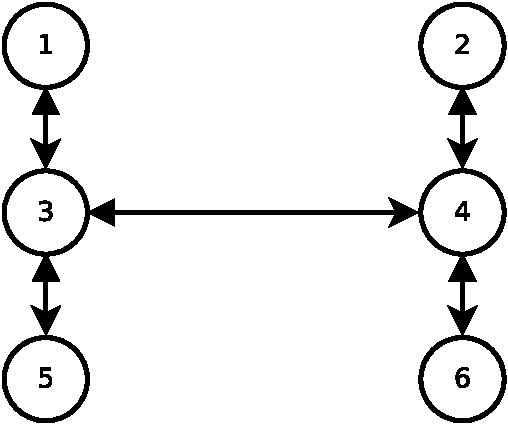
\includegraphics[scale=0.7]{fpp-proof-scheme.pdf}
    \caption{Schéma dôkazu ekvivalencie tvrdení z vety \ref{th:fpp_props}}
    \label{fig:fpp_props_scheme}
\end{figure}
Obrázok \ref{fig:fpp_props_scheme} znázorňuje schému dôkazu ekvivalencie týchto šiestich tvrdení.
Treba si dávať pozor na to, že ''platné'' tvrdenie znamená ''tvrdenie, odvodené z axiomatického systému PP1 až PP4''.
Preto neprehlásime duálne tvrdenia ihneď za ekvivalentné, nakoľko napríklad tvrdenie, že počet bodov je presne rovný $n^2 + n + 1$ pre nejaké fixné $n$, sa nedá odvodiť priamo z axiomatického systému.
Na druhej strane, duálne implikácie sa dajú prehlásiť za ekvivalentné ihneď.

\paragraph{$(1) \Longrightarrow (3)$ (a duálne $(2) \Longrightarrow (4)$):} Daná implikácia je očividná z dôvodu, že tvrdenie (1) hovorí o \emph{všetkých} priamkach, a tvrdenie (3) o existencii \emph{aspoň jednej} takej priamky.

\paragraph{$(3) \Longrightarrow (4)$ (a duálne $(4) \Longrightarrow (3)$):} 
Nech existuje priamka $L$ s presne $n+1$ bodmi $Q_1, \ldots Q_{n+1}$. 
Z PP3 vyplýva, že musí existovať bod mimo priamky $L$, označme si ho $P$. 
Z PP1 potom musia existovať $n+1$ priamok spájajúcich body  $Q_1, \ldots Q_{n+1}$ s~bodom $P$. 
Čiže bodom $P$ prechádza aspoň $n+1$ priamok. 
Ostáva už len dokázať, že cez daný bod neprechádza žiadna ďalšia priamka. 

Sporom, nech existuje priamka $K$, prechádzajúca bodom $P$. 
Z PP2 musí mať práve jeden spoločný bod s priamkou $L$. 
Sú tu dve možnosti: buď spoločným bodom priamok $L$ a $K$ je jeden z bodov $Q_1, \ldots Q_{n+1}$ alebo je to nejaký iný bod na priamke~$L$. 
V prvom prípade by došlo ku porušeniu PP2, keďže cez dva rôzne body $P$ a $Q_i$ by museli prechádzať dve rôzne priamky. 
V druhom prípade by došlo ku porušeniu pôvodného predpokladu, že priamka $L$ má práve $n+1$ bodov.

V skutočnosti sme práve dokázali silnejšie tvrdenie: \emph{bodom, ležiacim mimo priamky, ktorá má $m$ bodov, prechádza práve $m$ priamok} (a aj duálne ku nemu tvrdenie: \emph{priamka, neobsahujúca bod, ktorým prechádza $m$ priamok, obsahuje práve $m$ bodov}).

\paragraph{$(3) \Longrightarrow (1)$ (a duálne $(4) \Longrightarrow (2)$):} 
Nech existuje priamka $L$ s presne $n+1$ bodmi $Q_1, \ldots Q_{n+1}$. 
Z PP3 existujú štyri body $A, B, C$ a $D$ vo všeobecnej polohe, čiže aspoň dva z nich neležia na priamke $L$.
BUNV sú to $A$ a $B$.
Nakoľko dané body neležia na priamke $L$, prechádza cez ne práve $n+1$ priamok (viď tvrdenie dokázané vyššie).
Z toho vyplýva, že každá priamka, neobsahujúca $A$ alebo $B$, prechádza práve $n+1$ bodmi.
Ostáva už len dokázať, že aj priamka, spájajúca body $A$ a $B$, má tiež presne $n+1$ bodov.

Priamka $AC$ neobsahuje v sebe bod $B$ (lebo body $A,B,C$ a $D$ sú vo všeobecnej polohe), čiže tiež má presne $n+1$ bodov. 
Bod $D$ neleží na priamke $AC$, čiže im prechádza práve $n+1$ priamok.
Taktiež, bod $D$ neleží na priamke $AB$, čiže priamka $AB$ má presne $n+1$ bodov.

\paragraph{$(3) \Longrightarrow (5)$ (a duálne $(4) \Longrightarrow (6)$):}
Nech existuje priamka $L$ s $n+1$ bodmi $Q_1, \ldots Q_{n+1}$ a bod $P$ mimo tejto priamky (analogicky s predchádzajúcimi úvahami). 
Tvrdíme, že všetky body roviny sú obsiahnuté na priamkach $L, Q_1 P, \ldots Q_{n+1} P $.
Sporom, nech existuje bod $R$ mimo týchto priamok.
Potom musí existovať priamka $RP$, ktorá by porušila počet priamok, ktoré prechádzajú cez bod $P$.

Máme už dokázanú implikáciu $(3) \Longrightarrow (1)$, takže platí, že všetky priamky majú práve $n+1$ bodov.
Priamky $ Q_1 P, \ldots Q_{n+1} P $ majú spoločný bod $P$, čiže z PP2 zvyšné body musia mať rôzne.
Z toho už ľahko dopočítame celkový počet bodov: $(n+1) (n) + 1 = n^2 + n + 1$.

\paragraph{$(5) \Longrightarrow (3)$ (a duálne $(6) \Longrightarrow (4)$):}
Nech projektívna rovina má presne $n^2 + n + 1$ bodov.
Vezmime si niektorú priamku a označme počet jej bodov ako $m+1$.
Potom, z už dokázanej implikácie $(3) \Longrightarrow (5)$ vyplýva, že projektívna rovina má práve $m^2 + m + 1$ bodov.
Z toho plynie, že $m = n$, čím je dôkaz ukončený.
\end{proof}
\end{toreview}


\begin{definition}{(Kombinatorická definícia FPP)}\\
Konečná projektívna rovina rádu $n$ je $BIBD(v, k, \lambda)$ s parametrami:
$$v = n^2 + n + 1, k = n + 1, \lambda = 1$$
\end{definition}

\begin{theorem}
\label{th:fpp_bibd}
Kombinatorická a axiomatická definície konečnej projektívnej roviny sú ekvivalentné. 
\end{theorem}

\begin{toreview}
\begin{exercise}
Dokážte vetu \ref{th:fpp_bibd}.
\end{exercise}
\end{toreview}

\begin{definition}

Matica $C = (c_{ij})$ typu $n \times m$, kde $n \geq 4, m \geq 4$ a $c_{ij} \in \set{1, \ldots, n}$,  
má latinskú vlastnosť, ak ľubovoľná podmatica z dvoch stĺpcov matice $C$ nemá rovnaké riadky. Formálne,

$$\forall (i, j) \neq (k, l): (c_{ij}, c_{il}) \neq (c_{jk}, c_{jl})$$

Navyše, ak podmatica matice $C$, tvorená prvými dvomi stĺpcami, obsahuje postupne všetky dvojice čísel $\set{1, \ldots, n}$
v lexikografickom poradí, tak ju voláme matica s latinskou vlastnosťou v normálnom tvare.
\end{definition}

\begin{lemma}
\label{lm:ols_lp}
Nech $n \geq 3, t \geq 2$. Potom množina $t$ navzájom ortogonálnych latinských štvorcov rádu $n$ existuje práve vtedy,
keď existuje matica typu $n^2 \times (t+2)$ s latinskou vlastnosťou v normálnom tvare.
\end{lemma}
\begin{toreview}
\begin{construction}
Nech máme maticu typu $n^2 \times (t+2)$ s latinskou vlastnosťou v normálnom tvare.
Potom stĺpec $i+2$ udáva po riadkoch hodnoty políčok $i$-tého latinského štvorca.
Prevod z množiny ortogonálnych latinských štvorcov ku matici s latinskou vlastnosťou je z toho očividný.
\end{construction}
\begin{proof}
Nech máme maticu $M$ typu $n^2 \times (t+2)$ s latinskou vlastnosťou v normálnom tvare.
Treba overiť, že konštrukciou zostrojené matice sú latinskými štvorcami a potom či sú aj ortogonálne.
Prvé dva stĺpce matice $M$ obsahujú všetky usporiadané dvojice z $\{1, \ldots, n\}^2$.
V normálnom tvare zodpovedajú súradniciam v latinských štvorcoch, na ktoré sa umiestnia hodnoty z príslušného riadku.

Porovnaním prvého a $(i + 2)$-ého stĺpca matice $M$ z latinskej vlastnosti plynie, že v $i$-tom skonštruovanom štvorci na každom riadku sú zastúpené všetky hodnoty z množiny $\{1, \ldots, n\}$.
Podobne, porovnaním druhého a $(i + 2)$-ého stĺpca matice $M$ plynie to isté aj pre stĺpce $i$-tého skonštruovaného štvorca.
Čiže nami vykonštruované matice spĺňajú definíciu latinských štvorcov.

Ortogonalita $i$-tého a $j$-tého latinských štvorcov plynie priamo z porovnania príslušných stĺpcov $i+2$ a $j+2$ matice $M$ (viď definíciu ortogonality \ref{def:ols}).

Dôkaz opačného smeru konštrukcie je z toho už zrejmý.

\end{proof}
\end{toreview}

\begin{theorem}
\label{th:fpp_ols}
Existencia konečnej projektívnej roviny rádu $n$ je ekvivalentná s existenciou $(n-1)$ navzájom ortogonálnych latinských štvorcov rádu $n$.
\end{theorem}
\begin{toreview}
\begin{construction}
Nech existuje konečná projektívna rovina radu $n$.
Potom z vety \ref{th:fpp_props} má $n^2 + n + 1$ bodov a priamok.
Označme si priamky $\mathbb{X}_1$ až $\mathbb{X}_{n^2 + n + 1}$.
Označme si body na priamke $\mathbb{X}_1$ ako $x_1$ až $x_{n+1}$ a body mimo priamky ako $y_1$ až $y_{n^2}$.
Označme si priamky, odlišné od $\mathbb{X}_1$, na ktorých leží bod $x_{i}$ ako $L_{i, 1}$ až $L_{i, n}$.

Definujme si maticu $C$ typu $n^2 \times (n+1)$ tak, že $C_{i, j} = k \Longleftrightarrow y_i \in L_{j, k}$.
Potom matica $C$ má latinskú vlastnosť a z nej vieme podľa konštrukcie z lemy \ref{lm:ols_lp} zostrojiť množinu $(n-1)$ ortogonálnych latinských štvorcov radu $n$.

Konštrukcia pre opačný smer je z toho už zrejmá.
\end{construction}
\begin{proof}
Treba ukázať že nami definícia matice $C$ je korektná v zmysle, že pre každé $i$ a $j$ existuje práve jedno vhodné $k$ (z PP1), a že takto skonštruovaná matica má latinskú vlastnosť.
Technické detaily dôkazu ponechávame čitateľovi ako samostatné cvičenie \ref{ex:fpp_ols}.
\end{proof}

\begin{exercise}
\label{ex:fpp_ols}
Dokážte správnosť konštrukcie z vety \ref{th:fpp_ols}.
\end{exercise}

\end{toreview}

\begin{toreview}
\begin{corollary}
Ak $n$ je mocninou prvočísla, tak existuje konečná projektívna rovina rádu $n$.
\end{corollary}
\begin{proof}
Nech $n$ je mocninou prvočísla. Potom z vety \ref{thm:stevens} vyplýva existencia $n-1$ navzájom ortogonálnych latinských štvorcov radu $n$, z čoho podľa vety \ref{th:fpp_ols} vyplýva existencia konečnej projektívnej roviny radu $n$.
\end{proof}
\end{toreview}


\begin{hypothesis}
Ak existuje konečná projektívna rovina rádu $n$, tak $n$ je mocninou prvočísla.
\end{hypothesis}


\begin{toreview}

\begin{theorem_hard}{(Desarguesova\footnote{meno \emph{Desargues} sa číta ako [dezarg]} veta)}\\
\label{th:desargue}
%Если два треугольника расположены на плоскости таким образом, что прямые, соединяющие соответственные вершины треугольников, проходят через одну точку, то три точки, в которых пересекаются продолжения трёх пар соответственных сторон треугольников, лежат на одной прямой.
Ak dva trojuholníky sú umiestnené na (euklidovskej) rovine tak, že priamky, spájajúce príslušné dvojice vrcholov, prechádzajú spoločným bodom, tak tri body, v ktorých sa pretínajú predĺženia (t.j. priamky) troch dvojíc príslušných strán trojuholníkov, sú kolineárne (viď obrázok \ref{img:desargue}).
\end{theorem_hard}

\begin{figure}
    \centering
    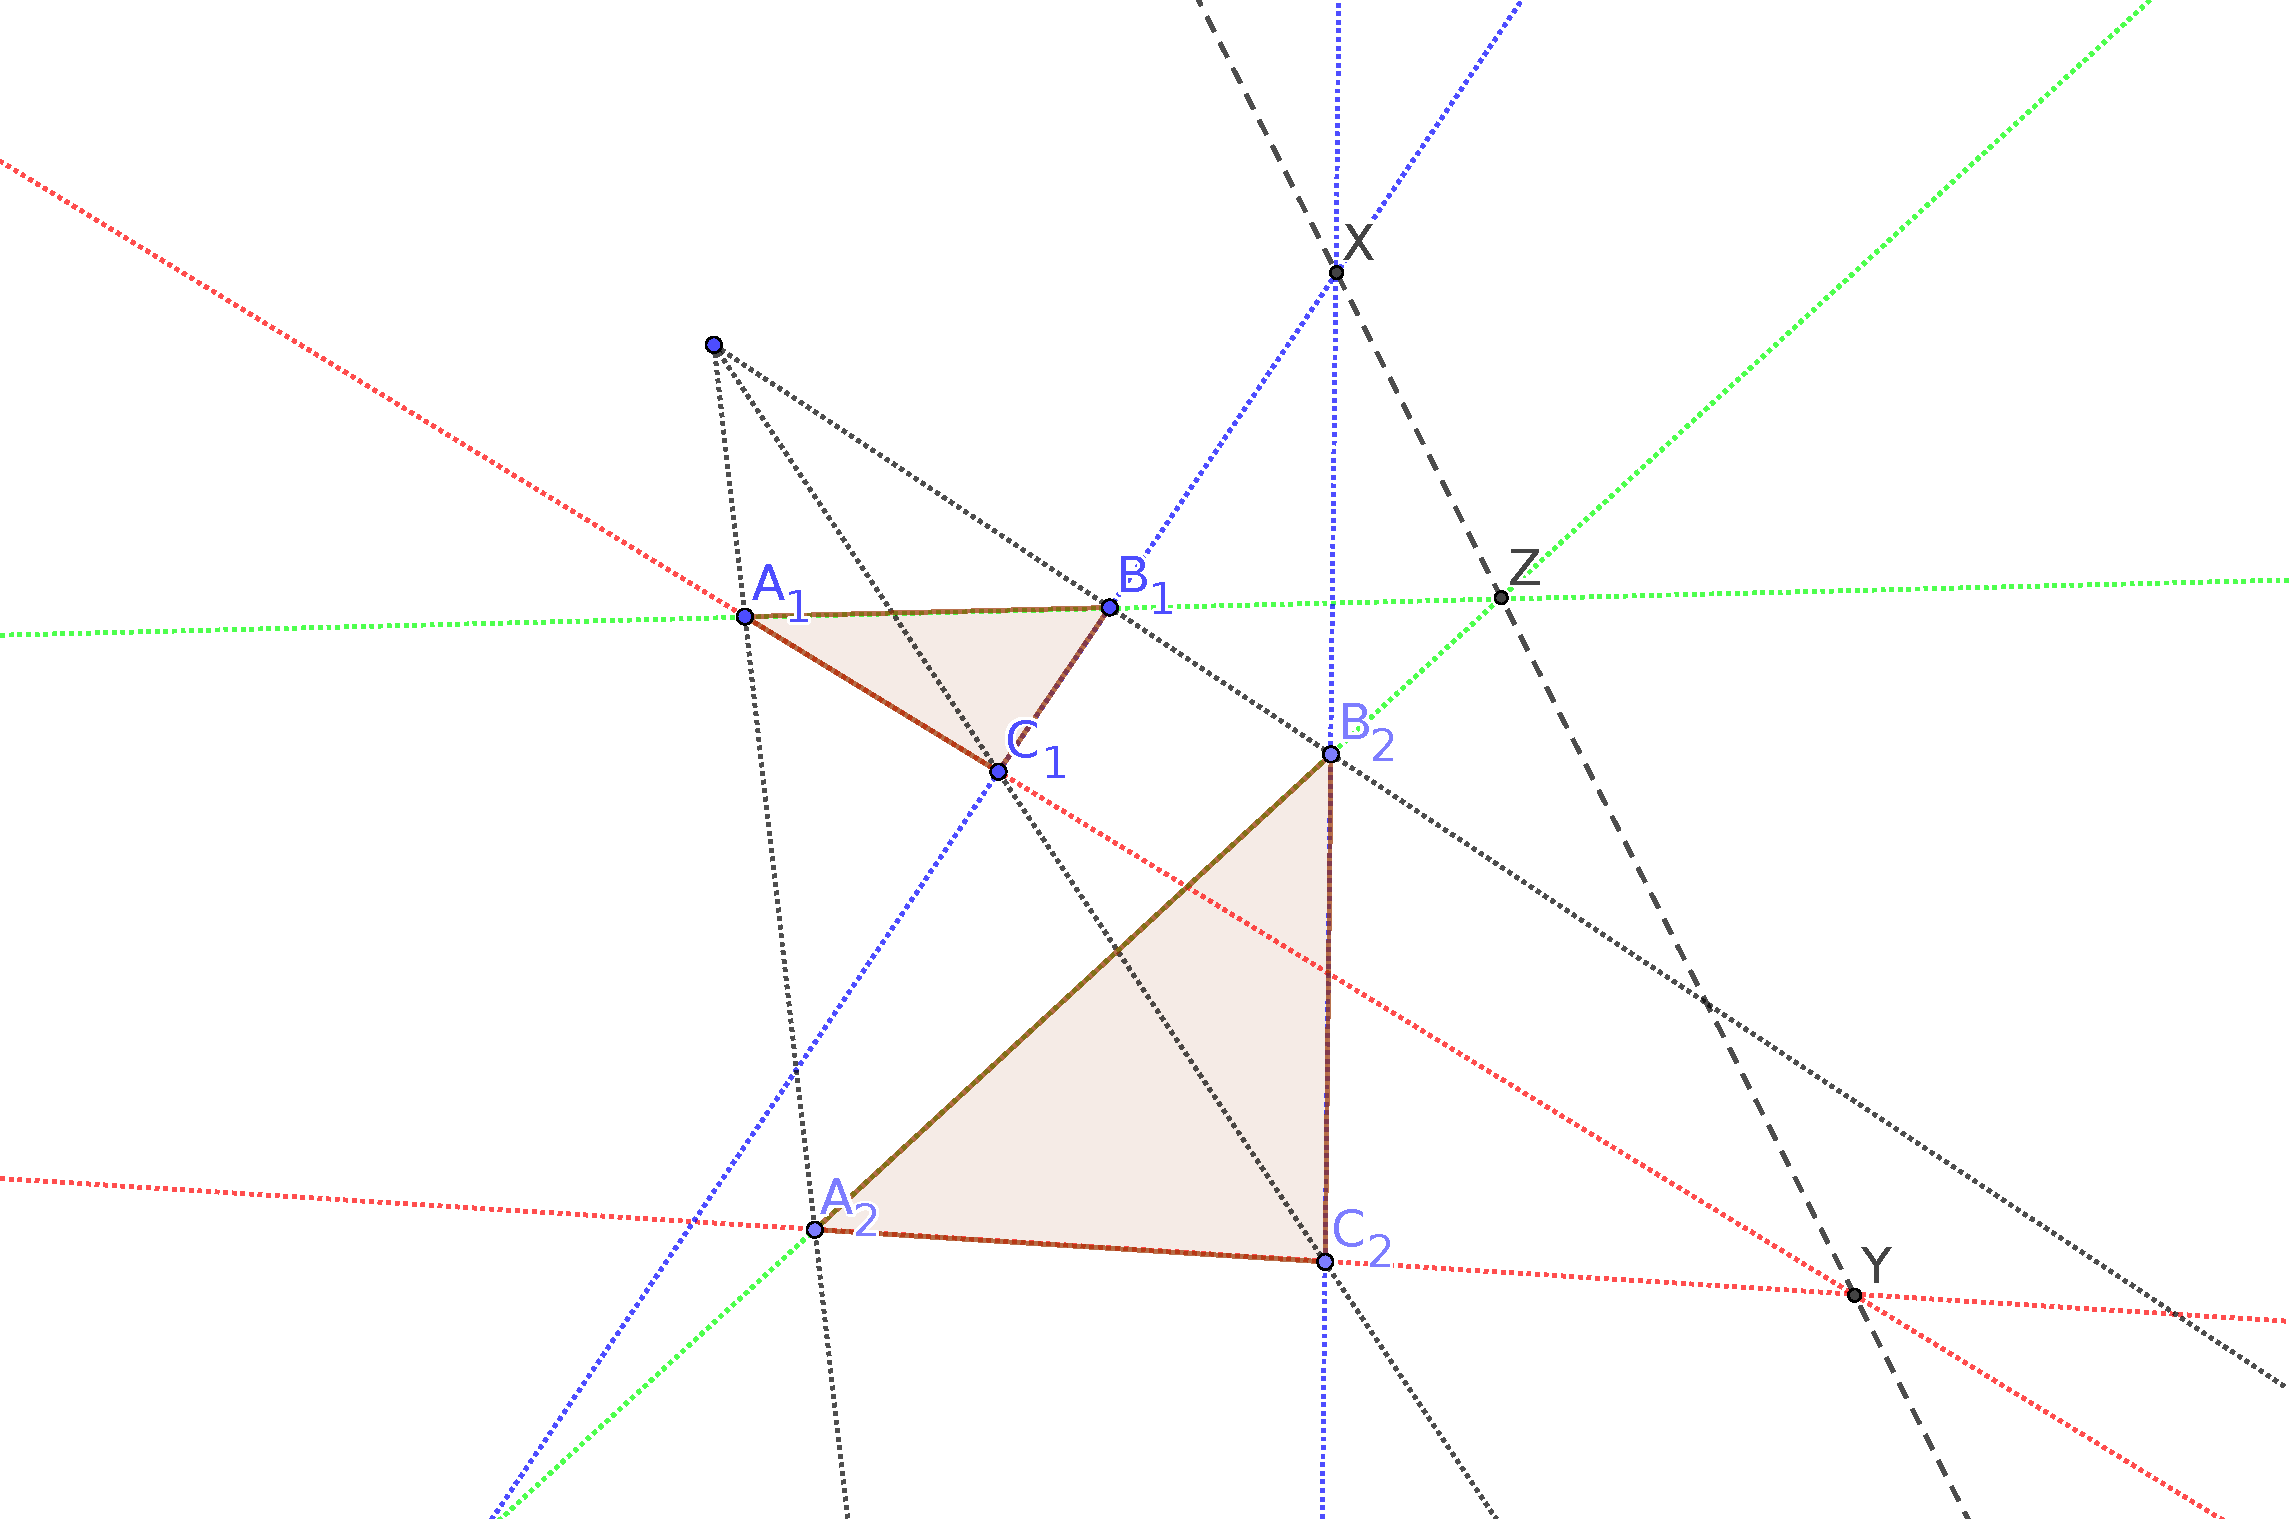
\includegraphics[width=\textwidth]{geogebra-export3.pdf}
    \caption{Ukážka Desarguesovej vety (\ref{th:desargue}). Priesečníky príslušných priamok (body $X$, $Y$ a $Z$) sú kolineárne.}
    \label{img:desargue}
\end{figure}

\end{toreview}

\section{Steinerovské systémy trojíc, zovšeobecnenia}

\begin{definition}
Blokové plány typu $BIBD(v, 3, 1)$ sa volajú Steinerovské systémy trojíc (angl. \emph{Steiner triplet system}, skrátene STS).
\end{definition}

\begin{remark}
Existencia STS je ekvivalentná s existenciou rozkladu kompletného grafu $K_v$ na trojuholníky.
\end{remark}

\begin{theorem}
\label{th:sts_nec}
Ak $v$ je počet objektov STS, tak $v \equiv 1 \mod 6$ alebo $v \equiv 3 \mod 6$.
\end{theorem}

\begin{theorem_hard}{(Kirkman)}\\
Ak $v$ spĺňa podmienky z vety \ref{th:sts_nec}, tak existuje STS s práve $v$ objektmi.
\end{theorem_hard}

\begin{theorem}{(Projektívne STS)\footnote{\TODO treba dôkaz?}}\\
Nech $X := \left(\mathbb{Z}_2\right)^{n+1} - \set{\vec{0}}$ je množina vektorov vektorového priestoru dimenzie $n+1$ nad poľom $\mathbb{Z}_2$ bez nulového vektora a 
$\mathcal{B} := \set{\set{\vec{x}, \vec{y}, \vec{z}} ~|~ \vec{x} + \vec{y} + \vec{z} = \vec{0}}$.
Potom dvojica $(X, \mathcal{B})$ je STS. Alternatívne, množina priamok projektívnej roviny $PG(2, n)$ tvorí STS.
\end{theorem}

\begin{theorem}{(Afinné STS)\footnote{\TODO treba dôkaz?}}\\
Nech $X := \left(\mathbb{Z}_3\right)^{n}$ je množina vektorov vektorového priestoru dimenzie $n$ nad poľom $\mathbb{Z}_3$. 
Nech $\mathcal{B} := \set{\set{\vec{x}, \vec{y}, \vec{z}} ~|~ \vec{x} + \vec{y} + \vec{z} = \vec{0}}$. Potom 
dvojica $(X, \mathcal{B})$ je STS.
\end{theorem}

\begin{theorem}{(Karteziansky súčin STS)}\\
Nech dvojice $(X, \mathcal{B})$ a $(Y, \mathcal{C})$ sú STS. Potom dvojica $(X \times Y, \mathcal{D})$, kde:
\begin{enumerate}
    \item $y \in Y, \set{b_1, b_2, b_3} \in \mathcal{B} \Longrightarrow \set{(b_1, y), (b_2, y), (b_3, y)} \in \mathcal{D}$
    \item $x \in X, \set{c_1, c_2, c_3} \in \mathcal{C} \Longrightarrow \set{(x, c_1), (x, c_2), (x, c_3)} \in \mathcal{D}$
    \item $\set{b_1, b_2, b_3} \in \mathcal{B}, \set{c_1, c_2, c_3} \in \mathcal{C}, \phi \in S_3 \Longrightarrow 
            \set{(b_1, c_{\phi(1)}), (b_2, c_{\phi(2)}), (b_3, c_{\phi(3)})} \in \mathcal{D}$ (kde $\phi$ je permutácia veľkosti $3$) 
\end{enumerate}

Potom $(X \times Y, \mathcal{D})$ je STS.
\end{theorem}


\begin{theorem}{(Vzťah STS a grupoidov)}\\
Nech $(X, \mathcal{B})$ je STS. Potom množina $X$ s binárnou operáciou $\ast$, definovanou nasledovne:
\begin{align*}
    \forall \set{x,y,z} \in \mathcal{B}:\\
    x\ast y = y \ast x = z\\ 
    x \ast z = z \ast x = y\\ 
    y\ast z = z \ast y = x\\
    x \ast x = x
\end{align*}

je idempotentný komutatívny grupoid. 
\end{theorem}


\begin{theorem}{(($2v +1$)-konštrukcia STS)}\\
Nech $(X, \mathcal{B})$ je STS a $(X', \mathcal{B}')$ je jeho disjunktná izomorfná kópia (t.j. $X \cap  X' = \varnothing$). Obraz prvku $x$ v tomto izomorfizme budeme značiť $x'$. 
Nech prvok $\infty \notin X \cup X'$.
Potom dvojica $(Y, \mathcal{C})$, kde $Y := X \cup X' \cup \set{\infty}$ a $\mathcal{C} := \mathcal{B} 
\cup \set{\set{x, y', z'} ~|~ \set{x,y,z}\in \mathcal{B}} 
\cup \set{\set{x, x', \infty} ~|~ x \in X}$, je STS.    
\end{theorem}

\TODO Paschovo prepnutie

\begin{theorem}{Wilson-Schreiberova konštrúkcia}\\
	Nech $n \equiv \pm 1 \pmod6$ je také celé číslo, že číslo $-2$ má v grupe $(\mathbb{Z}^*_n, \cdot)$ párny rád. Potom existuje STS rádu $n + 2$.
\end{theorem}

\begin{proof}
	Uvažujme všetky neusporiadané trojice $\langle a, b, c \rangle$ takých prvkov $\mathbb{Z}_n$, že $a + b + c = 0$. Tieto trojice sú troch typov:
	\begin{enumerate}
		\item $\langle a, b, c \rangle$, $a$, $b$, $c$ sú navzájom rôzne,
		\item $\langle a, b, c \rangle = \langle a, a, -2a \rangle$,
		\item $\langle a, b, c \rangle = \langle 0, 0, 0 \rangle$.
	\end{enumerate}
	Nech multiplikatívny rád čísla $-2$ modulo $n$ je $2r$. Zoberme dva nové prvky $\beta,\ \gamma \notin Z_n$. Pre fixné $a \in \mathbb{Z}_n - \{0\}$ si zoberme neusporiadané trojice druhého typu
	
	$$\langle              a,              a,  -2          a \rangle,$$
	$$\langle  -2          a,  -2          a, (-2)^2       a \rangle,$$
	$$\langle (-2)^2       a, (-2)^2       a, (-2)^3       a \rangle,$$
	$$\langle (-2)^3       a, (-2)^3       a, (-2)^4       a \rangle,$$
	$$\vdots$$
	$$\langle (-2)^{2r - 2}a, (-2)^{2r - 2}a, (-2)^{2r - 1}a \rangle,$$
	$$\langle (-2)^{2r - 1}a, (-2)^{2r - 1}a,              a \rangle = \langle (-2)^{2r - 1}a, (-2)^{2r - 1}a, (-2)^{2r}a \rangle.$$
	Pre $i \in \{0, 1, \dots, r-1\}$, trojicu $\langle (-2)^{2i}a, (-2)^{2i}a, (-2)^{2i + 1}a \rangle$ nahradíme trojicou $\langle (-2)^{2i}a, \alpha, (-2)^{2i + 1}a \rangle$ a trojicu $\langle (-2)^{2i + 1}a, (-2)^{2i + 1}a, (-2)^{2i + 2}a \rangle$ nahradíme trojicou $\langle (-2)^{2i}a, \alpha, (-2)^{2i + 1}a \rangle$. Dostaneme teda trojice typu
	\begin{align*}
	\langle              a,              a,  -2          a \rangle \quad \rightarrow& \quad \langle              a,         \alpha,  -2          a \rangle,\\
	\langle  -2          a,  -2          a, (-2)^2       a \rangle \quad \rightarrow& \quad \langle  -2          a,          \beta, (-2)^2       a \rangle,\\
	\langle (-2)^2       a, (-2)^2       a, (-2)^3       a \rangle \quad \rightarrow& \quad \langle (-2)^2       a,         \alpha, (-2)^3       a \rangle,\\
	\langle (-2)^2       a, (-2)^2       a, (-2)^3       a \rangle \quad \rightarrow& \quad \langle (-2)^2       a,          \beta, (-2)^3       a \rangle,\\
	\vdots&\\
	\langle (-2)^{2r - 2}a, (-2)^{2r - 2}a, (-2)^{2r - 1}a \rangle \quad \rightarrow& \quad \langle (-2)^{2r - 2}a,         \alpha, (-2)^{2r - 1}a \rangle,\\
	\langle (-2)^{2r - 1}a, (-2)^{2r - 1}a,              a \rangle \quad \rightarrow& \quad \langle (-2)^{2r - 1}a,          \beta,              a \rangle.
	\end{align*}
	Pokiaľ nám ostala ešte nejaká trojica $\langle b, b, -2b \rangle$ typu 2, tento postup s ňou zopakujeme, pokým všetky trojice typu dva takto nenahradíme.
	Nakoniec trojicu $\langle 0, 0, 0 \rangle$ nahradíme trojicou $\langle 0, \alpha, \beta \rangle$. Všetky trojice typu 1 ponecháme. Všetky nové trojice obsahujú tri rôzne prvky, už len ukážeme, že tvoria STS $(X, \mathcal{B})$ s nosnou množinou $X = \mathbb{Z}_n \cup \{\alpha, \beta \}$.
	
	Zoberme si ľubovoľnú dvojicu prvkov $a,\ b \in X$. Ak $\{ a, b \} = \{ \alpha, \beta \}$, tak sa $\{a, b\}$ nachádza v práve jednej trojici $\{0, \alpha, \beta \}$. Pokiaľ $a = \alpha$ a $b \in \mathbb{Z}_n$, tak $\alpha$ sa vyskytuje len v trojiciach typu 2. V nich sa $b$ vyskytuje iba v trojiciach $\langle b, b, -2b \rangle$ a $\langle (-2)^{-1}b, (-2)^{-1}b, b \rangle$. Práve jednu z nich sme prerobili na trojicu obsahujúcu $\alpha$, $b$. Prípad $a = \beta$, $b \in \mathbb{Z}_n$ je podobný.
	
	Pokiaľ $a \ne b \in \mathbb{Z}_n$, tak nech $c = - a - b$. Pokiaľ $a \ne c \ne b$, tak $\{a, b, c\}$ je jediná trojica obsahujúca $\{a, b\}$. Inak BUNV $c = a$. Potom $b = -2a$ a prvky $a$ a $-2a$ sa nachádzajú spolu v práce jednej trojici spolu s buď $\alpha$, alebo $\beta$.
\end{proof}

\begin{theorem_hard}{Wilson-Schreiberova konštrúkcia (všeobecnejšia)}\\
	Nech $n \equiv \pm 1 \pmod{6}$ a nech $A$ je Abelovská grupa rádu $n$, v ktorej $-2$ má párny multiplikatívny rád. Potom existuje STS rádu $n + 2$. 
\end{theorem_hard}

Táto veta využíva, že každá Abelovská grupa sa dá zapísať (vzhľadom na izomorfizus) ako súčin cyklických grúp. Pomocou nich možno definovať $-2$ ako $(-2,-2, \dots, -2)$, násobenie a multiplikatívny rád.

\TODO Boséova konštrukcia

\TODO Skolemova konštrukcia

\TODO Cyklické STS

\TODO Symetrické $v_3$-konfigurácie (čiastočné STS)

\begin{hypothesis}
Každý bezmostový kubický graf má 6 1-faktorov takých, že každá hrana grafu leží v práve 2 z nich.
\end{hypothesis}


\begin{definition}
Dvojica $(X, \mathcal{B})$, kde $\mathcal{B} \in \powerset(X)$, je $t-(v, k, \lambda)$-blokový plán (angl. \emph{$t$-design}), ak:
\begin{itemize}
    \item $\ssize{X} = v$
    \item $\forall B \in \mathcal{B}: \ssize{B} = k$
    \item každá $t$-tica objektov z $X$ sa vyskytuje v práve $\lambda$ blokoch z $\mathcal{B}$
\end{itemize}

Navyše, blokové plány typu $t-(v,k,1)$ budeme označovať ako $S(t,k,v)$.
\end{definition}

\begin{remark}
Existencia $t-(v,k,\lambda)$-blokového plánu je ekvivalentná s existenciou rozkladu $t$-uniformného $\lambda$-násobného hypergrafu na hyperklíky veľkosti $k$.
\end{remark}

\begin{remark}
STS s $v$ prvkami môžeme značiť ako $S(2,3,v)$.
\end{remark}

\begin{definition}
Blokové plány $S(3,4,v)$ voláme Steinerovské systémy štvoríc (angl. \emph{SQS})
\end{definition}

\begin{theorem_hard}

$\exists S(3,4,v) \Longleftrightarrow v \equiv 3,4 \mod 6$

\end{theorem_hard}


\begin{definition}
Blokové plány $S(4,5,v)$ voláme Steinerovské systémy pätíc
\end{definition}


\begin{theorem_hard}

$\exists S(4,5,v) \Longrightarrow v \equiv 4,5 \mod 6 \wedge v \not\equiv 4 \mod 5$

\end{theorem_hard}

\TODO konečné jednoduché grupy.
